\section{Balanced Truncation} \label{bt}
Balanced truncation is a method for model order reduction.
The goal of balanced truncation is to approximate a system using only the most relevant modes of the system.
The difference to POD is that the modes are not selected by the variance they capture but by the controllability and observability of the modes.
This is done by finding a coordinate transform.
\subsection{Balanceing Coordinate Transform} \label{balre}
To find a reduced order model using balanced truncation a orthonormal coordinate transform is applied: \(x = Tz\).
This yields a new system
\begin{gather}
\dot{z} = \hat{A}z + \hat{B}u \label{z1}\\
y = \hat{C}z + Du \label{z2} \\
\hat{A} = T^{-1}AT \quad \hat{B} = T^{-1}B \quad \hat{C} = CT \,.\label{red-sys-mat}
\end{gather}
The gramians of this ROM can be obtained by applying  (\ref{gram-obsv}) and (\ref{gram-ctrl}) to (\ref{red-sys-mat}).
This yields \(\hat{W}_c = T^{-1}W_cT^{-*}\) and \(\hat{W}_o = T^{*}W_oT\) with  \(T^{-*} := (T^{-1})^{*} := (T^{*})^{-1}\).
A requirement \(T\) has to satisfy is that it has to make the observability and controllability gramians of the ROM equal and diagonal
\begin{gather}
\hat{W}_c = \hat{W}_o = \Delta \\
\hat{W}_c \hat{W}_o = \Delta^{2} \\
T^{-1}W_cW_oT = \Delta^{2} \\
W_cW_oT = T\Delta^{2}  \,. \label{eigendec}
\end{gather}
Since \(\Delta\) is a diagonal matrix, (\ref{eigendec}) is equal to the eigendecomposition of \(W_cW_o\).
Therefore \(T\) contains the eigenvectors of \(W_cW_o\).
The values contained in \(\Delta\) are known as hankel singular values.
However \(T\) needs to be rescaled to make \(\hat{W}_c\) and \(\hat{W}_o\) equal.
Here \(T_u\) denotes the unscaled eigenvectors of this eigendecomposition that yields gramians that are not equal to each other
\begin{gather}
T_u^{-1}W_cT_u^{-*} = \Delta_c \label{e1}\\
T_u^{*}W_cT_u = \Delta_o  \,. \label{e2}
\end{gather}
Scaling \(T_u\) by some diagonal matrix \(\Delta_s\) results in \(\Delta_c = \Delta_o\)
\begin{gather}
\Delta_s = \Delta_c^{\frac{1}{4}}\Delta_o^{-\frac{1}{4}} \\
T = T_u \Delta_s  \,.
\end{gather}
Another important property of this transform is that the new coordinates are hierarchically ordered by observability and controllability.
It can be shown by deriving some unit vector \(\zeta\) that maximizes the controllability and observability
\begin{gather}
\zeta = arg\max \, \zeta^{*}W_cW_o\zeta \quad s.t. ||\zeta||_2^{2} = 1 \\
\frac{d}{d\zeta} \zeta^{*}W_cW_o\zeta - 2\lambda \zeta = 0  \,. \label{opt1}
\end{gather}
%https://www.matheplanet.com/matheplanet/nuke/html/viewtopic.php?rd2&topic=128338&start=0#p937673
As shown here \cite{170373} the remaining derivative can be solved in the following way
\begin{gather}
\frac{d}{dx} x^{*}Ax = 2Ax \,. \label{der-mat}
\end{gather}
This holds if \(A\) is symmetric. 
Here both \(W_c\) and \(W_o\) share the same set of eigenvectors (\ref{e1}) and (\ref{e2}), therefore they commute \cite{170371}.
This means that the product of \(W_c\) and \(W_o\) is also symmetric \cite{170372}.
Applying (\ref{der-mat}) to (\ref{opt1}) yields
\begin{gather}
W_cW_o\zeta = \lambda \zeta \,.
\end{gather}
Since \(\lambda\) is the Lagrange multiplier, it is a scalar. 
It is clear that \(\zeta\) is a eigenvector.
Since the eigenvalues in \(\Delta\) contain information about how much each eigenvector gets scaled by multiplying it with \(W_cW_o\) the eigenvectors can be ordered by controllability and observability.

\subsection{Mode Truncation}
Since the goal of balanced truncation is to find a ROM of rank \(r\) that approximates the original system of rank \(n\) with \(r << n\) it is necessary to truncate the balanced system.
This yields the following system:
\begin{gather}
\frac{d\tilde{x}}{dt} = \tilde{A}\tilde{X} + \tilde{B}u \\
y = \tilde{C}\tilde{x} + \tilde{D}u  \,.
\end{gather}
The new state vector \(\tilde{x}\) is defined as
\begin{gather}
\tilde{x} = \begin{bmatrix}
z_1 \\
\vdots \\
z_r
\end{bmatrix} \quad 
\tilde{z} = \begin{bmatrix}
z_{r+1} \\
\vdots \\
z_n
\end{bmatrix} \quad
z = \begin{bmatrix}
\tilde{x} \\
\tilde{z}
\end{bmatrix} \label{decomp-vecs}\\
T = \begin{bmatrix}
\Psi & T_t
\end{bmatrix} \quad
T^{-1} = S = \begin{bmatrix}
\Phi^{*} \\
S_t
\end{bmatrix}  \,. \label{decomp-mats}
\end{gather}
By substituting (\ref{decomp-vecs}) and (\ref{decomp-mats}) into the system in (\ref{z1}) and (\ref{z2}) the system becomes
\begin{gather}
\frac{d}{dt} \begin{bmatrix}
\tilde{x} \\
\tilde{z}
\end{bmatrix} = \begin{bmatrix}
\Phi^{*}A\Psi & \Phi^{*}AT_t \\
S_tA\Psi & S_tAT_t
\end{bmatrix} \begin{bmatrix}
\tilde{x} \\
\tilde{z}
\end{bmatrix}
+ \begin{bmatrix}
\Phi^{*}B \\
S_tB
\end{bmatrix} u \\
y = \begin{bmatrix}
C \Psi & CT_t
\end{bmatrix} \begin{bmatrix}
\tilde{x} \\
\tilde{z}
\end{bmatrix} + Du
 \,.
\end{gather}
However the only relevant part of this system is
\begin{gather}
\frac{d\tilde{x}}{dt} = \Phi^{*}A\Psi\tilde{x} + \Phi^{*}Bu \\
y = C\Psi\tilde{x} + Du  
\end{gather}
since this is the only part necessary to calculate \(\tilde{x}\)
\cite{brunton_kutz_2019e}.

\subsection{Computing Balanced Truncation}
Since the gramians for controllability and observability are too expensive to compute for large systems the so called empirical gramians are used as an approximation.
The empirical gramians are calculated by using the discrete-time system matrices from (\ref{disc-a}) and (\ref{disc-b})
\begin{gather}
\mathscr{C}_d = \begin{bmatrix}B_d & A_dB_d & \hdots & dA^{m_o -1}B_d\end{bmatrix} \\
\mathscr{O}_d = \begin{bmatrix}
C_d \\
C_dA_d \\
C_dA_d^{m_o - 1}
\end{bmatrix} \\
W_c^e = \mathscr{C}_d^{*}\mathscr{C}_d \\
W_o^e = \mathscr{O}_d^{*}\mathscr{O}_d \\
m_o, m_c << rank(A)  \,.
\end{gather}
Now these empirical gramians can be used for obtaining the balancing coordinate transform \cite{brunton_kutz_2019e}.

\subsection{State Space Representation from Heat Equation} \label{heat-ss}
To apply balanced truncation to the heat equation (\ref{eq-1d-h}) a state space representation of that system has to be found first.
Note that the system of ODEs resulting from FEM (\ref{almost-almost-ss}) resembles a state space representation
\begin{gather}
x := c \quad x_0 := c_0 \\
A := M^{-1}K \quad B:= I  \,.
\end{gather}
Since the system is realized as simulation all states can be accurately measured \(C := I\) and there is no feed through \(D := 0_{qm}\).
Now the already described steps for balanced truncation can be applied to the system.

Figure \ref{FIG-BT} shows a solution to heat equation using FEM and an approximation using BT with \(u(x, t) = 0, x_0 = 10000^{70\times1}, n = 70, n_{approx} = 10\).
\begin{figure}[H]
\centering
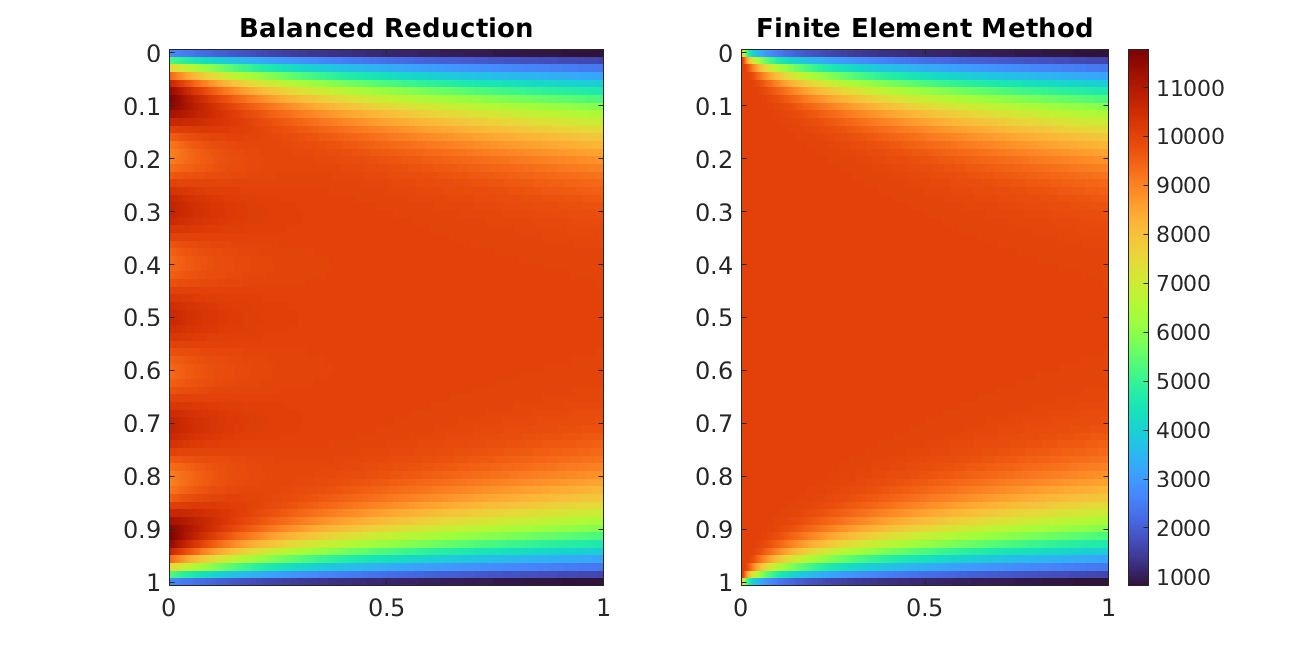
\includegraphics[ width=12.5cm]{images/bt}
\caption{FEM solution and BT approximation for heat equation}
\label{FIG-BT}
\end{figure}


